\chapter{Présentation de l'entreprise}
\chaptermark{Présentation Générale}
\minitoc
\newpage
 
\section{L’histoire de JungleBike}
Jungle Bike est une start up spécialisée dans le secteur du Vélo E-commerce dans la vente de matériels de vélos en ligne et aussi proposer à ses clients une facilitation de la réparation de leur vélos. \\
Elle est fondée en 2020 par Alice Battarel après ses trois années passées auprès de IBM en tant que consultante sénior en Innovation et Analytics avancée. Avec un capital de début de 500 €, Jungle Bike lance ses activités officiellement et fixe son siège au 15 Rue des Halles 75001, Paris. En 2020, Jungle Bike lance la mise en place de la plateforme d’aide à la réparation et de personnalisation du vélo. Cette plateforme répertoriera tous les réparateurs disponible que le client choisira en cas de problème de vélo.
Aujourd’hui Jungle Bike dispose de plus d’une vingtaine de partenaires fournisseur de pièces de vélo dont P2R, Comet.

\newpage
\section{Chiffres de JungleBike}
\begin{figure}[h]
\begin{center}
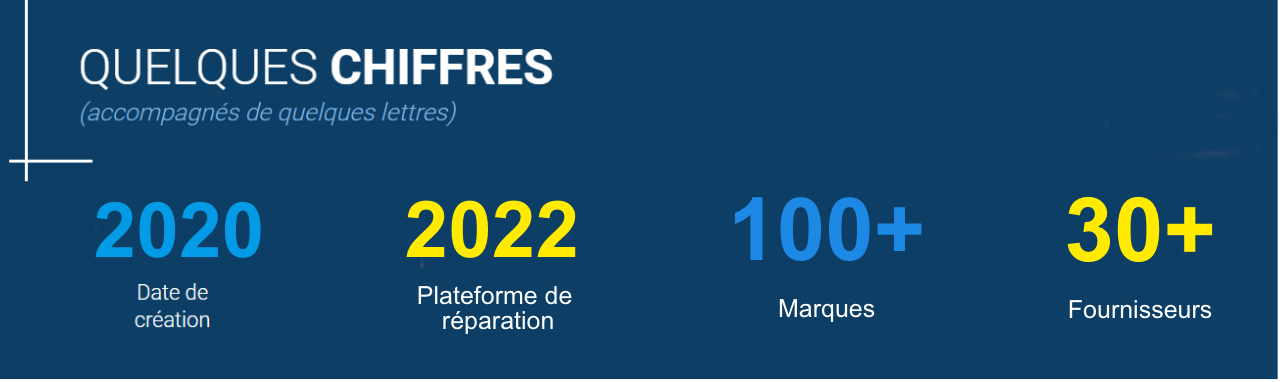
\includegraphics[width=15cm,height=6cm]{images/chiffres_jb.png}
\caption[Chiffres actuels sur l'évolution de JungleBike]{Chiffres actuels sur l'évolution de JungleBike}
\label{monlabel}
\end{center}
\end{figure}

\begin{figure}[h]
\begin{center}
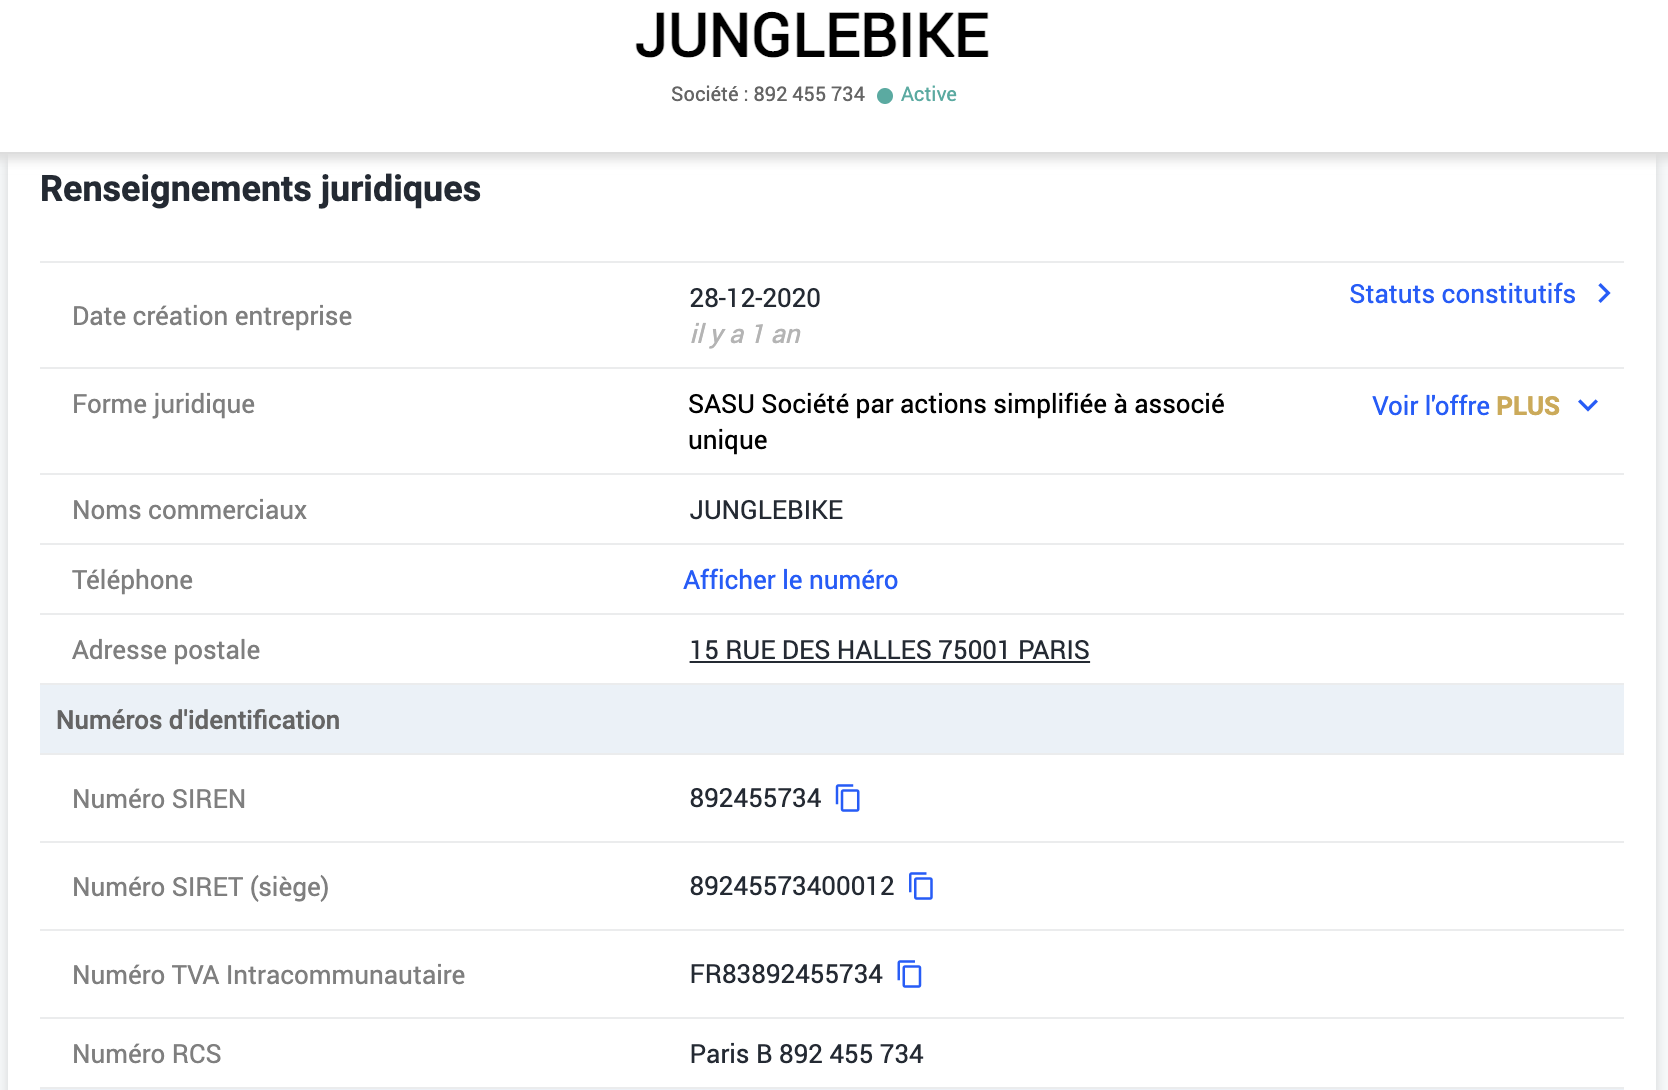
\includegraphics[width=15cm,height=9cm]{images/junglebike_juridique.png}
\caption[Informations juridique de JungleBike]{Informations juridique de JungleBike}
\label{monlabel}
\end{center}
\end{figure}
\newpage

\section{Les Services proposés}
\subsection{Accès des produits en ligne:}
Comme dit plus haut Jungle Bike reçoit des produits des fournisseurs en France ou à l'extérieur et les met à disposition des clients. Sur junglebike.fr les clients peuvent rechercher les produits par marque, origine et dimensions du produit. Pour toute commande effectuée, l'entrepôt basé au Mans (France) déclenche une livraison au client dans les 3 à 7 jours. Si le produit n’est pas conforme à l’attente du client, cette dernière peut procéder au retour de l’article dans le but d'être remboursé.:\\
	Dans le but d’avoir le stock synchronisé à celui du fournisseur, Jungle Bike dispose des algorithmes de mise à jour du stock. De nouveaux produits y sont régulièrement ajoutés dès qu’ils apparaissent chez le fournisseur.


\subsection{Enregistrement du vélo}
L’enregistrement du vélo est un service clé de Jungle Bike permettant d’identifier le modèle et ses différentes pièces que compose le vélo.\\
Toutes ces données permettront de faciliter la réparation ou la personnalisation du vélo. La plateforme dédiée à ce service permet au client de renseigner la marque, le type d’activité du vélo, période d’achat, taille des différentes parties du vélo. Le deuxième service de cette plateforme est que les clients pourront être mis en relation avec les réparateurs qui connaissent mieux les vélos pour la réparation ou la personnalisation.

\newpage

\section{Processus d’intégration de donnée et de mise en ligne des produits}
Tout d’abord avant qu’on ait accès à la fiche catalogue des produits des fournisseurs, JungleBike passe un contrat de vente des produits des marques du fournisseur.. 
\begin{figure}[h]
\begin{center}
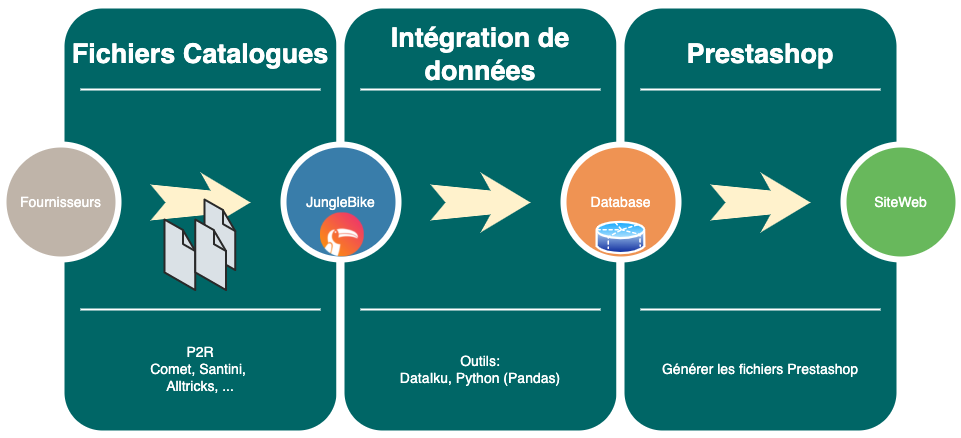
\includegraphics[width=15cm,height=8cm]{images/integration_steps.png}
\caption[Etapes d'intégration des produits]{Etapes d'intégration des produits}
\label{monlabel}
\end{center}
\end{figure}

\subsection{Récupérer le catalogue des produits}
Une fois la procédure de vente des produits du fournisseur validée, JungleBike reçoit les produits sous forme de données au format CSV, XLSX, SQL.
Extrait du fichier catalogue du fournisseur Mon Zoli Casque
\begin{figure}[h]
\begin{center}
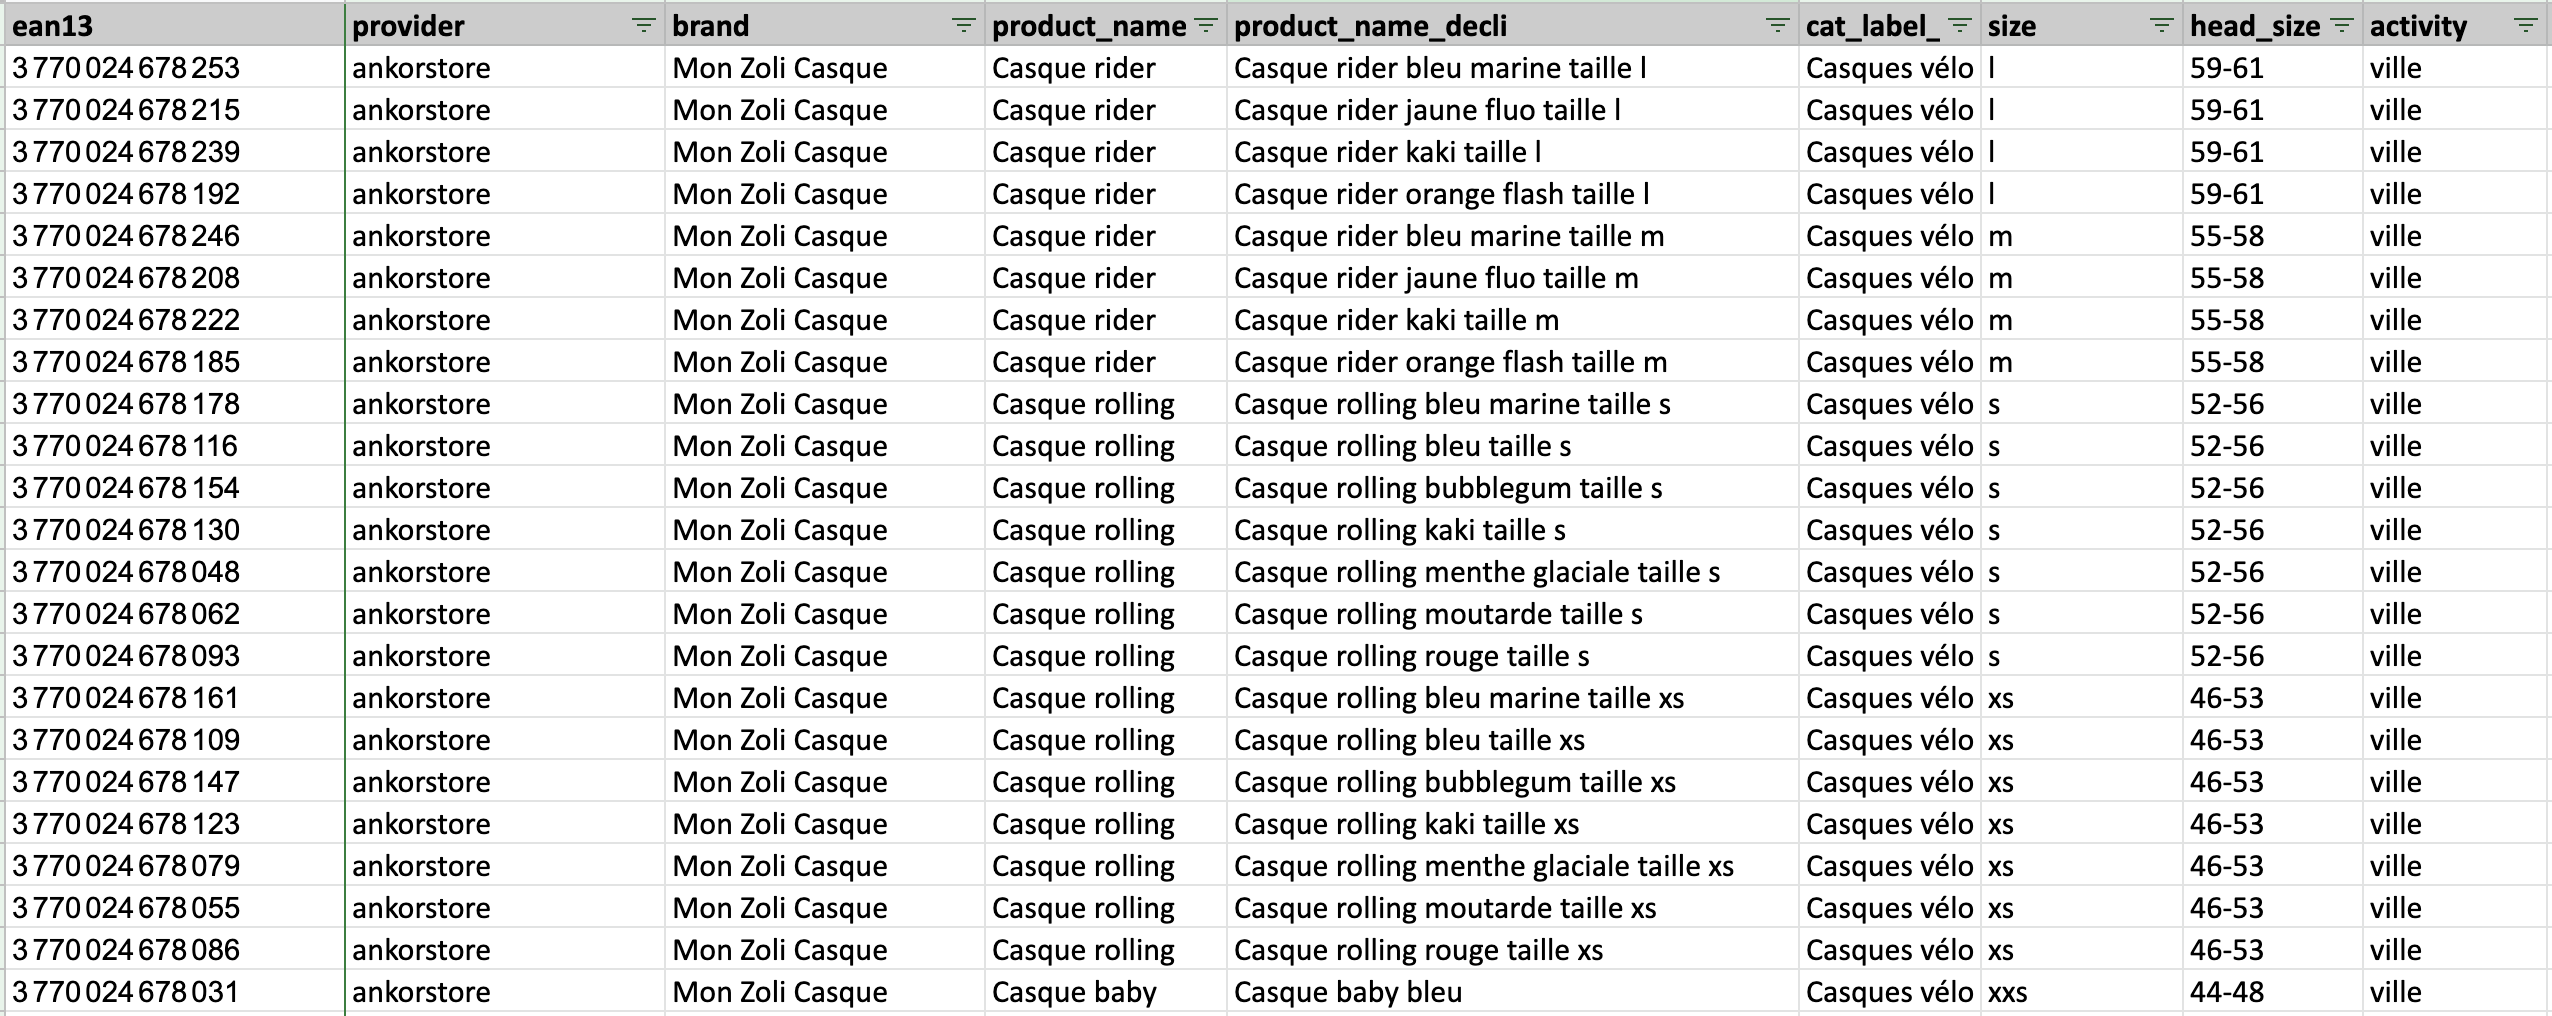
\includegraphics[width=15cm,height=8cm]{images/catalogue.png}
\caption[Exemple de données fournisseurs]{Exemple de données fournisseurs}
\label{monlabel}
\end{center}
\end{figure}
\subsection{Nettoyage et enrichissement et standardisation:}
Au début on nettoyait les produits avec Dataiku en créant des pipelines depuis l’extraction des données puis la transformation jusqu’au chargement dans un fichier csv.
Ensuite on a décidé de mettre en place un module permettant d'automatiser le processus ETL mais cette fois avec du python. Dans le processus de nettoyage, plusieurs étapes suivante sont nécessaire:\\
\begin{enumerate}
\item La catégorisation des produits conformément à toutes les catégories qu’on dispose. Un algorithme de catégorisation est donc appliqué en se basant sur le nom du produit.
\item Le nettoyage du nom du produit: les noms de produits comportant des tailles, couleurs, marques sont enlevés afin d’avoir un nom de produit sans d’autres informations.
\item Extraction des dimensions, couleurs, marque depuis le nom du produit ou depuis la colonne correspondante en suivant le référentiel de chaque colonne.
\item Création des identifiants unique de junglebike pour identifier chaque produit.
\end{enumerate}

\subsection{Mise en base:}
Une fois que les produits ont subi tout le processus de nettoyage et de standardisation, les produits sont chargés dans la base de donnée conçue à cet effet. Les différentes informations de chaque produit sont intégrées dans la table correspondante.
\subsection{Mise en ligne}
Pour rendre disponible ces produits en ligne, les produits sont chargés depuis la base puis subissent une transformation pour avoir le format spécifique à Prestashop. 
Cette dernière est uploadé sur le site afin d'être disponible sur le site.
\begin{figure}[h]
\begin{center}
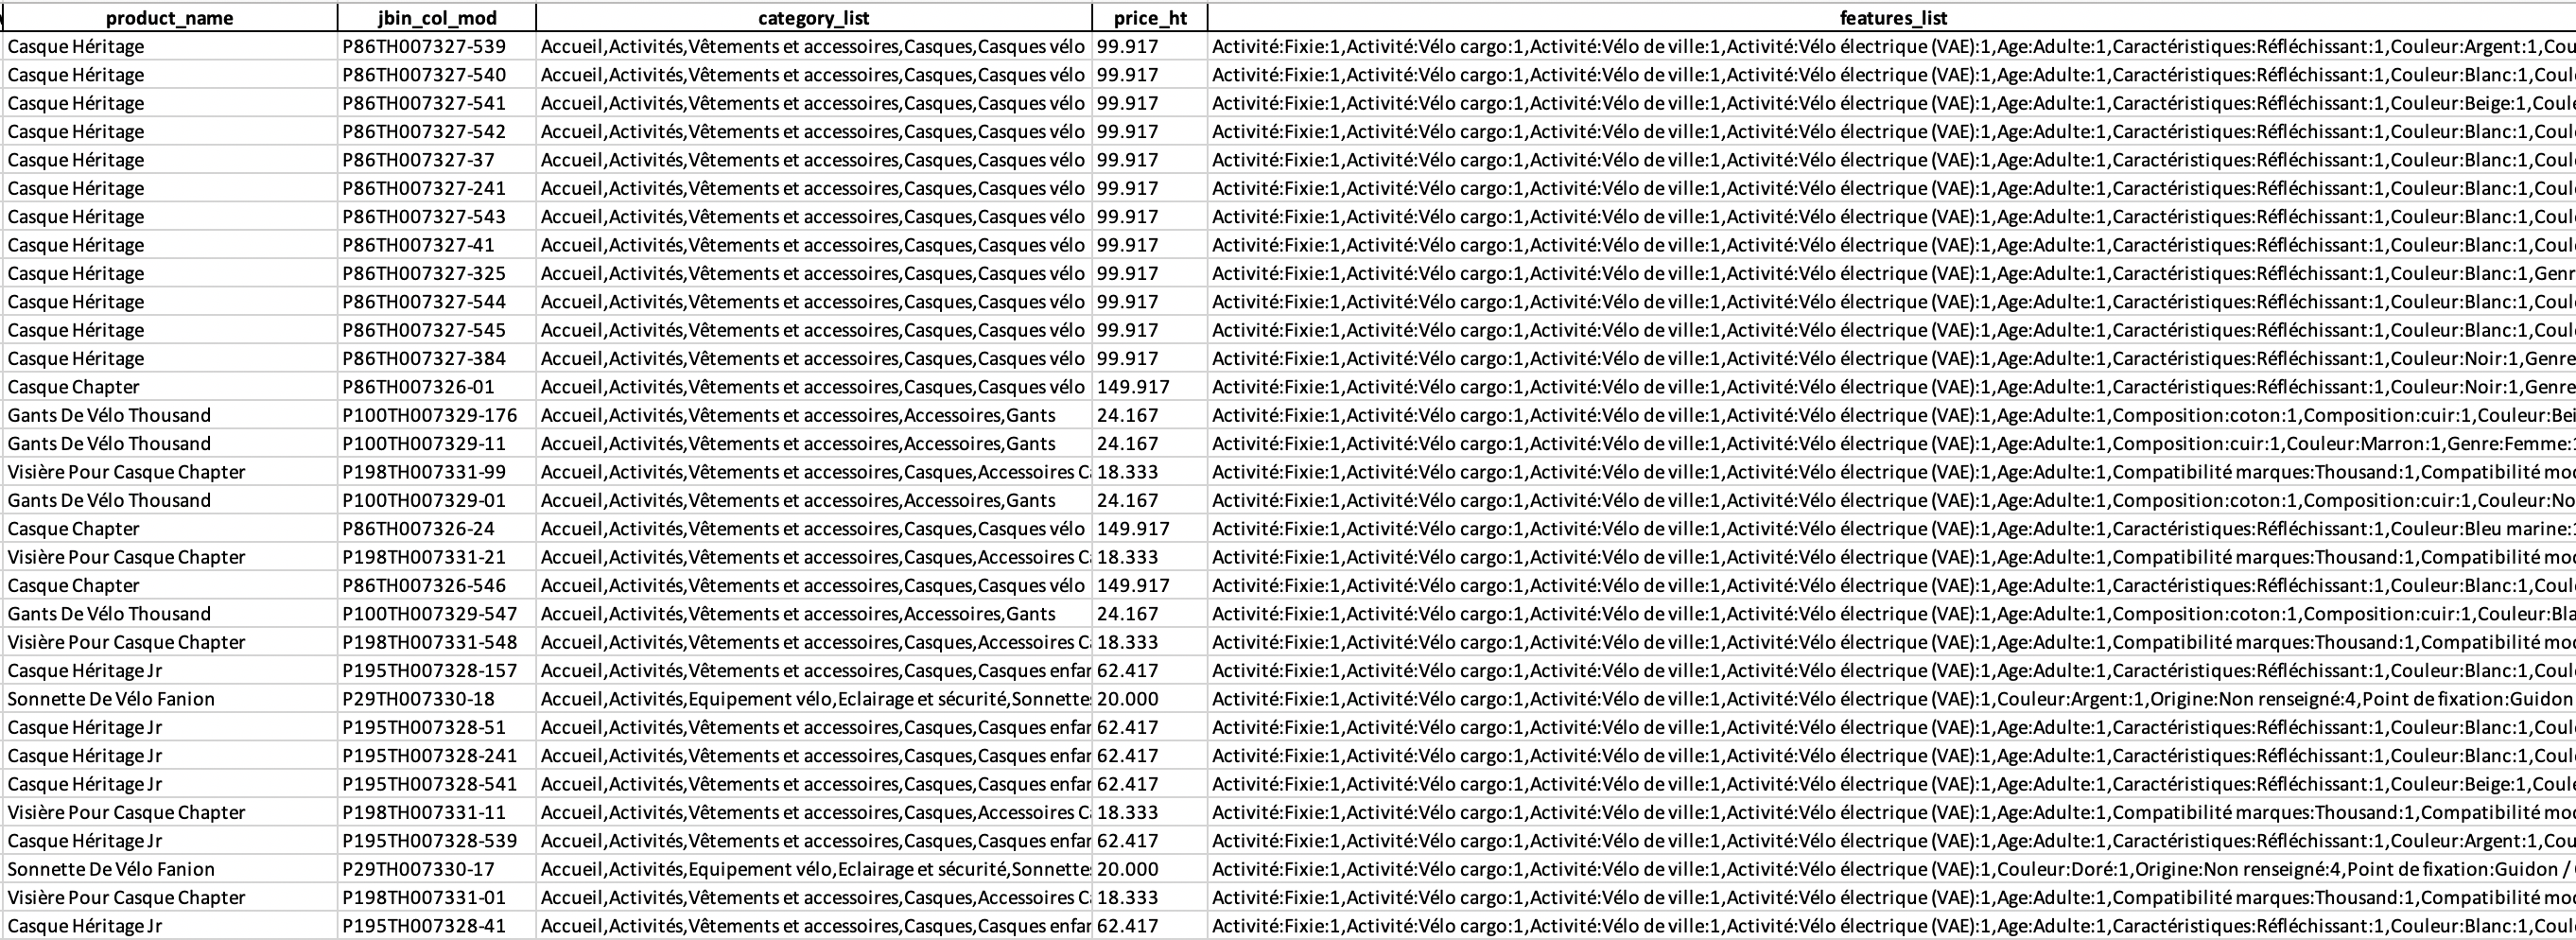
\includegraphics[width=15cm,height=8cm]{images/prestashop.png}
\caption[Aperçu des produits qui seront disponible en ligne]{Aperçu des produits qui seront disponible en ligne}
\label{monlabel}
\end{center}
\end{figure}
\newpage
\section{JungleBike en interne}

\subsection{L’ équipe d’accueil:}
L’équipe Data est composée de trois Data Scientist dont un intervenant externe. Mon collègue permanent travaille essentiellement sur la mise en place du module de compatibilité entre les produits et du module d’enregistrement des vélos. J’ai travaillé en premier sur le module d’automatisation d’intégration des données en base et sur le site. De plus, je suis amené à mettre en place l’algorithme de recommandation des articles du site en se basant sur les votes.

\subsection{Organisation de travail: le scrum Agile:}
 Scrum est une méthode agile pour la gestion de projet informatique et a pour objectif d’améliorer la productivité d’une équipe. C’est un cadre de travail au sein duquel les acteurs peuvent aborder des problèmes complexes et adaptatifs, en livrant de manière efficace et créative des produits tout en créant de la valeur ajoutée. Le sprint dure deux semaines et sur cette période chacun travaille sur une ou plusieurs tâches dans le but de fournir un résultat en fin de sprint. Le planificateur de tâche et de travail en équipe principale utilisé est Trello.

\subsection{Outils techniques:}
Dans le but de réaliser mes missions au sein de Transaction Connect, cette dernière a mis à ma disposition un ordinateur portable. Comme outils technique ou de communication on dispose entre autres de DBeaver, Pycharm, Slack, 
 Python, DataIku, Scikit Learn, Keras , Pytorch.








